\documentclass[aspectratio=169]{beamer}

\usepackage{tikz}
\usepackage{listings}
\usepackage[utf8,latin1]{inputenc}
\usepackage[natbibapa]{apacite}
\usepackage{multirow}
\usepackage{color, colortbl}
\usepackage{tcolorbox}

\makeatletter \def\newblock{\beamer@newblock} \makeatother

\beamertemplatenavigationsymbolsempty
\setbeamertemplate{itemize items}[circle]
\setbeamertemplate{section in toc}[circle]
\mode<beamer>{\setbeamercolor{math text displayed}{fg=iwmgray}}
\setbeamercolor{block body}{bg=iwmorange!50!white}
\setbeamercolor{block title}{fg=white, bg=iwmorange}

\definecolor{iwmorange}{RGB}{255,105,0}
\definecolor{iwmgray}{RGB}{67,79,79}
\definecolor{iwmblue}{RGB}{60,180,220}
\definecolor{iwmgreen}{RGB}{145,200,110}
\definecolor{iwmpurple}{RGB}{120,0,75}

\setbeamercolor{title}{fg=iwmpurple}
\setbeamercolor{frametitle}{fg=iwmpurple}
\setbeamercolor{structure}{fg=iwmpurple}
\setbeamercolor{normal text}{fg=iwmgray}
\setbeamercolor{author}{fg=iwmgray}
\setbeamercolor{date}{fg=iwmgray}

\lstset{language = R,%
  basicstyle = \ttfamily\color{iwmgray},
  frame = single,
  rulecolor = \color{iwmgray},
  commentstyle = \slshape\color{iwmgreen},
  keywordstyle = \bfseries\color{iwmgray},
  identifierstyle = \color{iwmpurple},
  stringstyle = \color{iwmblue},
  numbers = none,%left,numberstyle = \tiny,
  basewidth = {.5em, .4em},
  showstringspaces = false,
  emphstyle = \color{red!50!white}}

\setbeamercolor{graybox}{bg=iwmgray!30}
\newenvironment{colbox}[1][\textwidth]%
  {\begin{beamercolorbox}[wd=#1, rounded=true, shadow=true]{graybox}}
  {\end{beamercolorbox}}

\AtBeginSection[]{
  \frame{
    \tableofcontents[sectionstyle=show/hide, subsectionstyle=show/show/hide]}}

% \setbeamertemplate{headline}{
%  \begin{beamercolorbox}{section in head}
%    \vskip5pt\insertsectionnavigationhorizontal{\paperwidth}{}{}\vskip2pt
%  \end{beamercolorbox}
% }

\setbeamertemplate{footline}{\vskip-2pt\hfill\insertframenumber$\;$\vskip2pt}

\title{Summarizing results from a simulation study}
\author{Nora Wickelmaier\footnote{Parts of this slide set are a (modified)
version of slides accompanying Chapter 3 of the book by \citet{Strobl2024}}}
%\institute{Leibniz-Institut f\"ur Wissensmedien, T\"ubingen}
\date{Last modified: 2025-09-10}

\begin{document}

\begin{frame}{}
\thispagestyle{empty}
\titlepage
\end{frame}

% \begin{frame}{Outline}
% \tableofcontents
% \end{frame}

\begin{frame}{Estimator properties}
  \begin{itemize}
    \item One use of simulation studies it to examine the properties of
      statistical methods
    \item When we talk about ``statistical methods,'' we usually mean the
      estimation of one or more model parameters
    \item To evaluate the quality of point estimators, several relevant criteria
      exist\footnote{See, e.\,g., \url{https://en.wikipedia.org/wiki/Estimator}
      or any introductory statistics book}
      \begin{itemize}
        \item Unbiasedness
        \item Consistency
        \item Efficiency
        \item Suffiency
      \end{itemize}
    \item We will just look at two of them here: Unbiasedness and Consistency
  \end{itemize}
  \vfill
\end{frame}

\begin{frame}{Quality of point estimators}
{Unbiasedness}
  \begin{itemize}
    \item An estimator is called unbiased if the estimated values on average
      equal the true value
    \item If this only holds for large enough samples, the estimator is called
      asymptotically unbiased
    \item In our first simulation study, we examined the unbiasedness of the
      estimated slope coefficient in the regression model using plots and the
      bias
    \item Besides the bias, there are other statistics to examine unbiasedness
  \end{itemize}
  \vspace{.5cm}
  \[
      \widehat{Bias}_s = \frac{1}{niter}{\sum_{i = 1}^{niter}
      \left(\hat{\theta}_{is} - \theta_s\right)}
  \]
\end{frame}

\begin{frame}{Quality of point estimators}
{Unbiasedness}
\vspace{0.2cm}
\footnotesize
\begin{itemize}
  \item Percent bias
  \begin{equation*}
  \widehat{\%\,Bias}_s = \dfrac{\frac{1}{niter}{\sum_{i = 1}^{niter} (\hat{\theta}_{is} - \theta_s)}}{\theta_s}
  \end{equation*}
  \item Standardized bias
  \begin{equation*}
\widehat{stand\,Bias}_s = \dfrac{\frac{1}{niter}{\sum_{i = 1}^{niter} (\hat{\theta}_{is} - \theta_s)}}{se_s\left(\widehat{Bias}\right)}
  \end{equation*}
  \item Absolute bias
  \begin{equation*}
\widehat{abs\,Bias}_s = \frac{1}{niter}{\sum_{i = 1}^{niter} |\hat{\theta}_{is} - \theta_s|},
  \end{equation*}
  \item Mean squared error (MSE) / Root mean squared error (RMSE)
  \begin{equation*}
\widehat{MSE}_s = \frac{1}{niter}{\sum_{i = 1}^{niter} (\hat{\theta}_{is} -
    \theta_s)^2} \quad/\quad \widehat{RMSE}_s = \sqrt{\frac{1}{niter}{\sum_{i = 1}^{niter} (\hat{\theta}_{is} - \theta_s)^2}}
  \end{equation*}
\item[$\to$] For unbiased estimators, all of the discussed statistics should be
  close to 0
\end{itemize}
\end{frame}

\begin{frame}{Quality of point estimators}
{Consistency}
  \begin{columns}
    \begin{column}{.5\textwidth}
\begin{itemize}
  \item An estimator is consistent if the estimates scatter closer around the
    true value as the sample size increases
  \item If an estimator is consistent, it is also (asymptotically) unbiased
  \item The consistency of an estimator can be checked by graphically displaying
    the distribution of the individual estimates for different sample sizes
\end{itemize}
    \end{column}
    \begin{column}{.5\textwidth}
      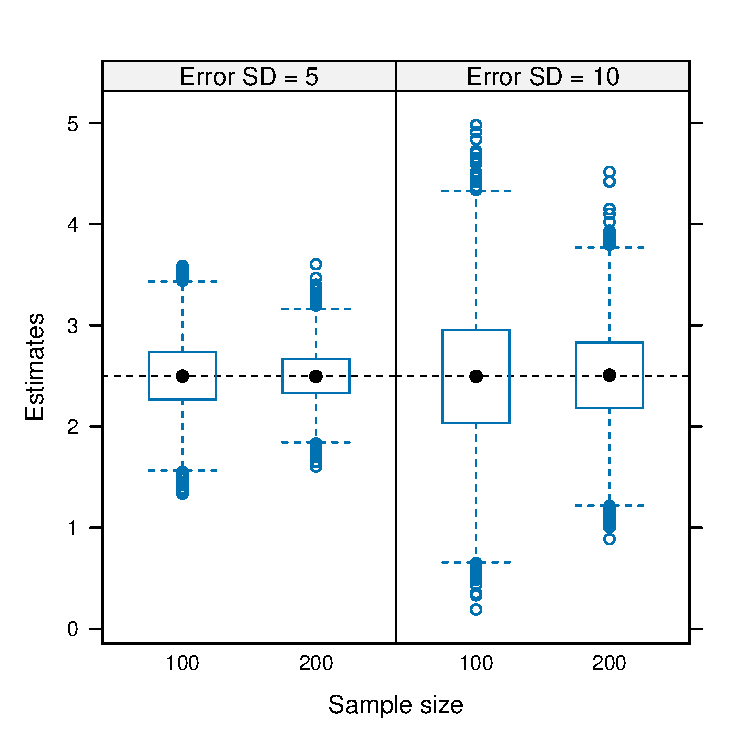
\includegraphics[scale = .57]{../figures/boxplot_simstudy_example1}
    \end{column}
  \end{columns}
\end{frame}

\begin{frame}{Quality of confidence intervals}
\begin{itemize}
  \item Confidence intervals (CIs) with a confidence level of e.g.~95\% can be
    constructed around point estimators
  \item That means, if we were to repeatedly collect samples and would calculate
    the confidence interval from each sample, about 95\% of the confidence
    intervals would cover the true value
  \item In a simulation study we can determine the actual proportion of
    confidence intervals that cover the true value
  \item This is called the estimated coverage probability
  \begin{equation*}
\widehat{CP}_s = \dfrac{\sum_{i = 1}^{niter} I(\theta_s \in CI_{is})}{niter},
\end{equation*}
\noindent where $I$ denotes the indicator function that takes the value 1 if the
event specified in parentheses occurs, and otherwise takes the value 0
\end{itemize}
\end{frame}

\begin{frame}{Simulation study to investigate estimator properties for nonnormal
  data}
  \begin{itemize}[<+->]
    \item Now, let us combine what we learned so far
    \item How does normality of data influence the estimation of the slope
      parameter in a simple regression?
    \item Create a simulation study to investigate unbiasedness and consistency
    \item What factors should we vary?
      \begin{itemize}
        \item Data generation: normal vs.\ nonnormal
        \item What nonnormal data generation should we use?
        \item Sample size $n$
        \item What test for normality should we pick?
        \item Anything else you would like to vary?
      \end{itemize}
    \item How can we quantify the biasedness of our parameter estimate?
    \item How can we determine if the estimator is consistent?
      %Confidence intervals?
  \end{itemize}
  \vfill
\end{frame}

\appendix
\begin{frame}{References}
%\begin{frame}[allowframebreaks]{References}
%\renewcommand{\bibfont}{\footnotesize}
\bibliographystyle{apacite}
\bibliography{../lit}
\end{frame}

\end{document}

